\documentclass[twoside]{book}

% Packages required by doxygen
\usepackage{fixltx2e}
\usepackage{calc}
\usepackage{doxygen}
\usepackage[export]{adjustbox} % also loads graphicx
\usepackage{graphicx}
\usepackage[utf8]{inputenc}
\usepackage{makeidx}
\usepackage{multicol}
\usepackage{multirow}
\PassOptionsToPackage{warn}{textcomp}
\usepackage{textcomp}
\usepackage[nointegrals]{wasysym}
\usepackage[table]{xcolor}

% Font selection
\usepackage[T1]{fontenc}
\usepackage[scaled=.90]{helvet}
\usepackage{courier}
\usepackage{amssymb}
\usepackage{sectsty}
\renewcommand{\familydefault}{\sfdefault}
\allsectionsfont{%
  \fontseries{bc}\selectfont%
  \color{darkgray}%
}
\renewcommand{\DoxyLabelFont}{%
  \fontseries{bc}\selectfont%
  \color{darkgray}%
}
\newcommand{\+}{\discretionary{\mbox{\scriptsize$\hookleftarrow$}}{}{}}

% Page & text layout
\usepackage{geometry}
\geometry{%
  a4paper,%
  top=2.5cm,%
  bottom=2.5cm,%
  left=2.5cm,%
  right=2.5cm%
}
\tolerance=750
\hfuzz=15pt
\hbadness=750
\setlength{\emergencystretch}{15pt}
\setlength{\parindent}{0cm}
\setlength{\parskip}{0.2cm}
\makeatletter
\renewcommand{\paragraph}{%
  \@startsection{paragraph}{4}{0ex}{-1.0ex}{1.0ex}{%
    \normalfont\normalsize\bfseries\SS@parafont%
  }%
}
\renewcommand{\subparagraph}{%
  \@startsection{subparagraph}{5}{0ex}{-1.0ex}{1.0ex}{%
    \normalfont\normalsize\bfseries\SS@subparafont%
  }%
}
\makeatother

% Headers & footers
\usepackage{fancyhdr}
\pagestyle{fancyplain}
\fancyhead[LE]{\fancyplain{}{\bfseries\thepage}}
\fancyhead[CE]{\fancyplain{}{}}
\fancyhead[RE]{\fancyplain{}{\bfseries\leftmark}}
\fancyhead[LO]{\fancyplain{}{\bfseries\rightmark}}
\fancyhead[CO]{\fancyplain{}{}}
\fancyhead[RO]{\fancyplain{}{\bfseries\thepage}}
\fancyfoot[LE]{\fancyplain{}{}}
\fancyfoot[CE]{\fancyplain{}{}}
\fancyfoot[RE]{\fancyplain{}{\bfseries\scriptsize Generated on Thu Mar 31 2016 22\+:27\+:27 for Test Project by Doxygen }}
\fancyfoot[LO]{\fancyplain{}{\bfseries\scriptsize Generated on Thu Mar 31 2016 22\+:27\+:27 for Test Project by Doxygen }}
\fancyfoot[CO]{\fancyplain{}{}}
\fancyfoot[RO]{\fancyplain{}{}}
\renewcommand{\footrulewidth}{0.4pt}
\renewcommand{\chaptermark}[1]{%
  \markboth{#1}{}%
}
\renewcommand{\sectionmark}[1]{%
  \markright{\thesection\ #1}%
}

% Indices & bibliography
\usepackage{natbib}
\usepackage[titles]{tocloft}
\setcounter{tocdepth}{3}
\setcounter{secnumdepth}{5}
\makeindex

% Hyperlinks (required, but should be loaded last)
\usepackage{ifpdf}
\ifpdf
  \usepackage[pdftex,pagebackref=true]{hyperref}
\else
  \usepackage[ps2pdf,pagebackref=true]{hyperref}
\fi
\hypersetup{%
  colorlinks=true,%
  linkcolor=blue,%
  citecolor=blue,%
  unicode%
}

% Custom commands
\newcommand{\clearemptydoublepage}{%
  \newpage{\pagestyle{empty}\cleardoublepage}%
}


%===== C O N T E N T S =====

\begin{document}

% Titlepage & ToC
\hypersetup{pageanchor=false,
             bookmarks=true,
             bookmarksnumbered=true,
             pdfencoding=unicode
            }
\pagenumbering{roman}
\begin{titlepage}
\vspace*{7cm}
\begin{center}%
{\Large Test Project }\\
\vspace*{1cm}
{\large Generated by Doxygen 1.8.9.1}\\
\vspace*{0.5cm}
{\small Thu Mar 31 2016 22:27:27}\\
\end{center}
\end{titlepage}
\clearemptydoublepage
\tableofcontents
\clearemptydoublepage
\pagenumbering{arabic}
\hypersetup{pageanchor=true}

%--- Begin generated contents ---
\chapter{Class Index}
\section{Class List}
Here are the classes, structs, unions and interfaces with brief descriptions\+:\begin{DoxyCompactList}
\item\contentsline{section}{\hyperlink{structBox}{Box} }{\pageref{structBox}}{}
\item\contentsline{section}{\hyperlink{classLightcone}{Lightcone} }{\pageref{classLightcone}}{}
\item\contentsline{section}{\hyperlink{structLightconeSettings}{Lightcone\+Settings} }{\pageref{structLightconeSettings}}{}
\item\contentsline{section}{\hyperlink{structParticle}{Particle} }{\pageref{structParticle}}{}
\item\contentsline{section}{\hyperlink{classSnapshot}{Snapshot} }{\pageref{classSnapshot}}{}
\item\contentsline{section}{\hyperlink{classTimer}{Timer} }{\pageref{classTimer}}{}
\end{DoxyCompactList}

\chapter{File Index}
\section{File List}
Here is a list of all files with brief descriptions\+:\begin{DoxyCompactList}
\item\contentsline{section}{\hyperlink{CosmicLightcone_8cpp}{Cosmic\+Lightcone.\+cpp} }{\pageref{CosmicLightcone_8cpp}}{}
\item\contentsline{section}{\hyperlink{Lightcone_8cpp}{Lightcone.\+cpp} }{\pageref{Lightcone_8cpp}}{}
\item\contentsline{section}{\hyperlink{Lightcone_8h}{Lightcone.\+h} }{\pageref{Lightcone_8h}}{}
\item\contentsline{section}{\hyperlink{Snapshot_8cpp}{Snapshot.\+cpp} }{\pageref{Snapshot_8cpp}}{}
\item\contentsline{section}{\hyperlink{Snapshot_8h}{Snapshot.\+h} }{\pageref{Snapshot_8h}}{}
\item\contentsline{section}{\hyperlink{Timer_8cpp}{Timer.\+cpp} }{\pageref{Timer_8cpp}}{}
\item\contentsline{section}{\hyperlink{Timer_8h}{Timer.\+h} }{\pageref{Timer_8h}}{}
\end{DoxyCompactList}

\chapter{Class Documentation}
\hypertarget{structBox}{}\section{Box Struct Reference}
\label{structBox}\index{Box@{Box}}


{\ttfamily \#include $<$Snapshot.\+h$>$}

\subsection*{Public Member Functions}
\begin{DoxyCompactItemize}
\item 
\hyperlink{structBox_aca78d7db44972bfa78d46b7bbc8796f6}{Box} ()
\item 
\hyperlink{structBox_aa8e9518bc21db23d43bac103a51004af}{Box} (double \hyperlink{structBox_a3527f292bb4bde18936b2dfc76097ea0}{x}, double \hyperlink{structBox_a4a11736337f490a1e0903c4f12badf05}{y}, double \hyperlink{structBox_adfc8262c4a354b354ef319e592980138}{z}, double \hyperlink{structBox_a52c7a693671af3a6b9e713c989c28a1b}{w})
\item 
\hyperlink{structBox_ac1f84c8bc4b686e4a20868a82e82a6b6}{Box} (double \hyperlink{structBox_a3527f292bb4bde18936b2dfc76097ea0}{x}, double \hyperlink{structBox_a4a11736337f490a1e0903c4f12badf05}{y}, double \hyperlink{structBox_adfc8262c4a354b354ef319e592980138}{z}, double \hyperlink{structBox_a52c7a693671af3a6b9e713c989c28a1b}{w}, double \hyperlink{structBox_a6ddf8580fc6085be5311720212d966f0}{h}, double \hyperlink{structBox_a512cdd18477dcf4b59df213935b9ad9d}{d})
\end{DoxyCompactItemize}
\subsection*{Public Attributes}
\begin{DoxyCompactItemize}
\item 
double \hyperlink{structBox_a3527f292bb4bde18936b2dfc76097ea0}{x}
\item 
double \hyperlink{structBox_a4a11736337f490a1e0903c4f12badf05}{y}
\item 
double \hyperlink{structBox_adfc8262c4a354b354ef319e592980138}{z}
\item 
double \hyperlink{structBox_a52c7a693671af3a6b9e713c989c28a1b}{w}
\item 
double \hyperlink{structBox_a6ddf8580fc6085be5311720212d966f0}{h}
\item 
double \hyperlink{structBox_a512cdd18477dcf4b59df213935b9ad9d}{d}
\end{DoxyCompactItemize}


\subsection{Constructor \& Destructor Documentation}
\hypertarget{structBox_aca78d7db44972bfa78d46b7bbc8796f6}{}\index{Box@{Box}!Box@{Box}}
\index{Box@{Box}!Box@{Box}}
\subsubsection[{Box}]{\setlength{\rightskip}{0pt plus 5cm}Box\+::\+Box (
\begin{DoxyParamCaption}
{}
\end{DoxyParamCaption}
)\hspace{0.3cm}{\ttfamily [inline]}}\label{structBox_aca78d7db44972bfa78d46b7bbc8796f6}
\hypertarget{structBox_aa8e9518bc21db23d43bac103a51004af}{}\index{Box@{Box}!Box@{Box}}
\index{Box@{Box}!Box@{Box}}
\subsubsection[{Box}]{\setlength{\rightskip}{0pt plus 5cm}Box\+::\+Box (
\begin{DoxyParamCaption}
\item[{double}]{x, }
\item[{double}]{y, }
\item[{double}]{z, }
\item[{double}]{w}
\end{DoxyParamCaption}
)\hspace{0.3cm}{\ttfamily [inline]}}\label{structBox_aa8e9518bc21db23d43bac103a51004af}
\hypertarget{structBox_ac1f84c8bc4b686e4a20868a82e82a6b6}{}\index{Box@{Box}!Box@{Box}}
\index{Box@{Box}!Box@{Box}}
\subsubsection[{Box}]{\setlength{\rightskip}{0pt plus 5cm}Box\+::\+Box (
\begin{DoxyParamCaption}
\item[{double}]{x, }
\item[{double}]{y, }
\item[{double}]{z, }
\item[{double}]{w, }
\item[{double}]{h, }
\item[{double}]{d}
\end{DoxyParamCaption}
)\hspace{0.3cm}{\ttfamily [inline]}}\label{structBox_ac1f84c8bc4b686e4a20868a82e82a6b6}


\subsection{Member Data Documentation}
\hypertarget{structBox_a512cdd18477dcf4b59df213935b9ad9d}{}\index{Box@{Box}!d@{d}}
\index{d@{d}!Box@{Box}}
\subsubsection[{d}]{\setlength{\rightskip}{0pt plus 5cm}double Box\+::d}\label{structBox_a512cdd18477dcf4b59df213935b9ad9d}
\hypertarget{structBox_a6ddf8580fc6085be5311720212d966f0}{}\index{Box@{Box}!h@{h}}
\index{h@{h}!Box@{Box}}
\subsubsection[{h}]{\setlength{\rightskip}{0pt plus 5cm}double Box\+::h}\label{structBox_a6ddf8580fc6085be5311720212d966f0}
\hypertarget{structBox_a52c7a693671af3a6b9e713c989c28a1b}{}\index{Box@{Box}!w@{w}}
\index{w@{w}!Box@{Box}}
\subsubsection[{w}]{\setlength{\rightskip}{0pt plus 5cm}double Box\+::w}\label{structBox_a52c7a693671af3a6b9e713c989c28a1b}
\hypertarget{structBox_a3527f292bb4bde18936b2dfc76097ea0}{}\index{Box@{Box}!x@{x}}
\index{x@{x}!Box@{Box}}
\subsubsection[{x}]{\setlength{\rightskip}{0pt plus 5cm}double Box\+::x}\label{structBox_a3527f292bb4bde18936b2dfc76097ea0}
\hypertarget{structBox_a4a11736337f490a1e0903c4f12badf05}{}\index{Box@{Box}!y@{y}}
\index{y@{y}!Box@{Box}}
\subsubsection[{y}]{\setlength{\rightskip}{0pt plus 5cm}double Box\+::y}\label{structBox_a4a11736337f490a1e0903c4f12badf05}
\hypertarget{structBox_adfc8262c4a354b354ef319e592980138}{}\index{Box@{Box}!z@{z}}
\index{z@{z}!Box@{Box}}
\subsubsection[{z}]{\setlength{\rightskip}{0pt plus 5cm}double Box\+::z}\label{structBox_adfc8262c4a354b354ef319e592980138}


The documentation for this struct was generated from the following file\+:\begin{DoxyCompactItemize}
\item 
\hyperlink{Snapshot_8h}{Snapshot.\+h}\end{DoxyCompactItemize}

\hypertarget{classLightcone}{}\section{Lightcone Class Reference}
\label{classLightcone}\index{Lightcone@{Lightcone}}


{\ttfamily \#include $<$Lightcone.\+h$>$}

\subsection*{Public Member Functions}
\begin{DoxyCompactItemize}
\item 
\hyperlink{classLightcone_a995eaddc1bd40670ba09c6d91314fcc7}{Lightcone} ()
\item 
void \hyperlink{classLightcone_a6cd0b42be0281e70a6ef5e6a2701f587}{set\+Lightcone} (\hyperlink{structLightconeSettings}{Lightcone\+Settings} settings)
\item 
void \hyperlink{classLightcone_a5439f4ef2e9b61101aecd07d4f516de9}{set\+Observer} (\hyperlink{structParticle}{Particle} obs)
\item 
void \hyperlink{classLightcone_a9245eee21d6b57b9d5bf0b1fcc918448}{set\+Label} (string str)
\item 
bool \hyperlink{classLightcone_a4b1c9b9d855cf08cdc4316ba9823d52c}{load\+Redshift\+Steps} ()
\item 
void \hyperlink{classLightcone_a105a489ed768bc9c29acd5239d993c96}{generate} ()
\item 
vector$<$ \hyperlink{structParticle}{Particle} $>$ \hyperlink{classLightcone_a5a9ed81cce84c6602ef722e0398f7f20}{get\+Segment} (\hyperlink{classSnapshot}{Snapshot} \&snap, double r\+Max, double r\+Min)
\item 
void \hyperlink{classLightcone_afcf40a6029a13ec619317b3eea792795}{write} ()
\item 
string \hyperlink{classLightcone_a5a7028a7c597d4a2f64410c0bff997fc}{get\+Setting\+String} ()
\end{DoxyCompactItemize}
\subsection*{Public Attributes}
\begin{DoxyCompactItemize}
\item 
string \hyperlink{classLightcone_a4abb9ce077488d3744e00b1ad4969299}{output\+File\+Path}
\end{DoxyCompactItemize}
\subsection*{Static Public Attributes}
\begin{DoxyCompactItemize}
\item 
static const int \hyperlink{classLightcone_aaa0aec147530ceafd1f6237b13e19268}{B\+O\+X\+\_\+\+W\+I\+D\+T\+H} = 500
\item 
static int \hyperlink{classLightcone_a82c274cc5d7d3db62e9e4b64a1fc11da}{T\+A\+O\+\_\+\+S\+T\+A\+R\+T\+I\+N\+G\+\_\+\+I\+D} = 1409
\item 
static string \hyperlink{classLightcone_a5e3e2f76c9a6230556cf82e170221d1f}{R\+E\+D\+S\+H\+I\+F\+T\+\_\+\+P\+A\+T\+H} = \char`\"{}\char`\"{}
\item 
static string \hyperlink{classLightcone_ad96b184f7878ceb27ed89aa6ee7fda0b}{O\+U\+T\+P\+U\+T\+\_\+\+P\+A\+T\+H} = \char`\"{}\char`\"{}
\end{DoxyCompactItemize}


\subsection{Constructor \& Destructor Documentation}
\hypertarget{classLightcone_a995eaddc1bd40670ba09c6d91314fcc7}{}\index{Lightcone@{Lightcone}!Lightcone@{Lightcone}}
\index{Lightcone@{Lightcone}!Lightcone@{Lightcone}}
\subsubsection[{Lightcone}]{\setlength{\rightskip}{0pt plus 5cm}Lightcone\+::\+Lightcone (
\begin{DoxyParamCaption}
{}
\end{DoxyParamCaption}
)}\label{classLightcone_a995eaddc1bd40670ba09c6d91314fcc7}


\subsection{Member Function Documentation}
\hypertarget{classLightcone_a105a489ed768bc9c29acd5239d993c96}{}\index{Lightcone@{Lightcone}!generate@{generate}}
\index{generate@{generate}!Lightcone@{Lightcone}}
\subsubsection[{generate}]{\setlength{\rightskip}{0pt plus 5cm}void Lightcone\+::generate (
\begin{DoxyParamCaption}
{}
\end{DoxyParamCaption}
)}\label{classLightcone_a105a489ed768bc9c29acd5239d993c96}
\hypertarget{classLightcone_a5a9ed81cce84c6602ef722e0398f7f20}{}\index{Lightcone@{Lightcone}!get\+Segment@{get\+Segment}}
\index{get\+Segment@{get\+Segment}!Lightcone@{Lightcone}}
\subsubsection[{get\+Segment}]{\setlength{\rightskip}{0pt plus 5cm}vector$<$ {\bf Particle} $>$ Lightcone\+::get\+Segment (
\begin{DoxyParamCaption}
\item[{{\bf Snapshot} \&}]{snap, }
\item[{double}]{r\+Max, }
\item[{double}]{r\+Min}
\end{DoxyParamCaption}
)}\label{classLightcone_a5a9ed81cce84c6602ef722e0398f7f20}
\hypertarget{classLightcone_a5a7028a7c597d4a2f64410c0bff997fc}{}\index{Lightcone@{Lightcone}!get\+Setting\+String@{get\+Setting\+String}}
\index{get\+Setting\+String@{get\+Setting\+String}!Lightcone@{Lightcone}}
\subsubsection[{get\+Setting\+String}]{\setlength{\rightskip}{0pt plus 5cm}string Lightcone\+::get\+Setting\+String (
\begin{DoxyParamCaption}
{}
\end{DoxyParamCaption}
)}\label{classLightcone_a5a7028a7c597d4a2f64410c0bff997fc}
\hypertarget{classLightcone_a4b1c9b9d855cf08cdc4316ba9823d52c}{}\index{Lightcone@{Lightcone}!load\+Redshift\+Steps@{load\+Redshift\+Steps}}
\index{load\+Redshift\+Steps@{load\+Redshift\+Steps}!Lightcone@{Lightcone}}
\subsubsection[{load\+Redshift\+Steps}]{\setlength{\rightskip}{0pt plus 5cm}bool Lightcone\+::load\+Redshift\+Steps (
\begin{DoxyParamCaption}
{}
\end{DoxyParamCaption}
)}\label{classLightcone_a4b1c9b9d855cf08cdc4316ba9823d52c}
\hypertarget{classLightcone_a9245eee21d6b57b9d5bf0b1fcc918448}{}\index{Lightcone@{Lightcone}!set\+Label@{set\+Label}}
\index{set\+Label@{set\+Label}!Lightcone@{Lightcone}}
\subsubsection[{set\+Label}]{\setlength{\rightskip}{0pt plus 5cm}void Lightcone\+::set\+Label (
\begin{DoxyParamCaption}
\item[{string}]{str}
\end{DoxyParamCaption}
)}\label{classLightcone_a9245eee21d6b57b9d5bf0b1fcc918448}
\hypertarget{classLightcone_a6cd0b42be0281e70a6ef5e6a2701f587}{}\index{Lightcone@{Lightcone}!set\+Lightcone@{set\+Lightcone}}
\index{set\+Lightcone@{set\+Lightcone}!Lightcone@{Lightcone}}
\subsubsection[{set\+Lightcone}]{\setlength{\rightskip}{0pt plus 5cm}void Lightcone\+::set\+Lightcone (
\begin{DoxyParamCaption}
\item[{{\bf Lightcone\+Settings}}]{settings}
\end{DoxyParamCaption}
)}\label{classLightcone_a6cd0b42be0281e70a6ef5e6a2701f587}
\hypertarget{classLightcone_a5439f4ef2e9b61101aecd07d4f516de9}{}\index{Lightcone@{Lightcone}!set\+Observer@{set\+Observer}}
\index{set\+Observer@{set\+Observer}!Lightcone@{Lightcone}}
\subsubsection[{set\+Observer}]{\setlength{\rightskip}{0pt plus 5cm}void Lightcone\+::set\+Observer (
\begin{DoxyParamCaption}
\item[{{\bf Particle}}]{obs}
\end{DoxyParamCaption}
)}\label{classLightcone_a5439f4ef2e9b61101aecd07d4f516de9}
\hypertarget{classLightcone_afcf40a6029a13ec619317b3eea792795}{}\index{Lightcone@{Lightcone}!write@{write}}
\index{write@{write}!Lightcone@{Lightcone}}
\subsubsection[{write}]{\setlength{\rightskip}{0pt plus 5cm}void Lightcone\+::write (
\begin{DoxyParamCaption}
{}
\end{DoxyParamCaption}
)}\label{classLightcone_afcf40a6029a13ec619317b3eea792795}


\subsection{Member Data Documentation}
\hypertarget{classLightcone_aaa0aec147530ceafd1f6237b13e19268}{}\index{Lightcone@{Lightcone}!B\+O\+X\+\_\+\+W\+I\+D\+T\+H@{B\+O\+X\+\_\+\+W\+I\+D\+T\+H}}
\index{B\+O\+X\+\_\+\+W\+I\+D\+T\+H@{B\+O\+X\+\_\+\+W\+I\+D\+T\+H}!Lightcone@{Lightcone}}
\subsubsection[{B\+O\+X\+\_\+\+W\+I\+D\+T\+H}]{\setlength{\rightskip}{0pt plus 5cm}const int Lightcone\+::\+B\+O\+X\+\_\+\+W\+I\+D\+T\+H = 500\hspace{0.3cm}{\ttfamily [static]}}\label{classLightcone_aaa0aec147530ceafd1f6237b13e19268}
\hypertarget{classLightcone_ad96b184f7878ceb27ed89aa6ee7fda0b}{}\index{Lightcone@{Lightcone}!O\+U\+T\+P\+U\+T\+\_\+\+P\+A\+T\+H@{O\+U\+T\+P\+U\+T\+\_\+\+P\+A\+T\+H}}
\index{O\+U\+T\+P\+U\+T\+\_\+\+P\+A\+T\+H@{O\+U\+T\+P\+U\+T\+\_\+\+P\+A\+T\+H}!Lightcone@{Lightcone}}
\subsubsection[{O\+U\+T\+P\+U\+T\+\_\+\+P\+A\+T\+H}]{\setlength{\rightskip}{0pt plus 5cm}string Lightcone\+::\+O\+U\+T\+P\+U\+T\+\_\+\+P\+A\+T\+H = \char`\"{}\char`\"{}\hspace{0.3cm}{\ttfamily [static]}}\label{classLightcone_ad96b184f7878ceb27ed89aa6ee7fda0b}
\hypertarget{classLightcone_a4abb9ce077488d3744e00b1ad4969299}{}\index{Lightcone@{Lightcone}!output\+File\+Path@{output\+File\+Path}}
\index{output\+File\+Path@{output\+File\+Path}!Lightcone@{Lightcone}}
\subsubsection[{output\+File\+Path}]{\setlength{\rightskip}{0pt plus 5cm}string Lightcone\+::output\+File\+Path}\label{classLightcone_a4abb9ce077488d3744e00b1ad4969299}
\hypertarget{classLightcone_a5e3e2f76c9a6230556cf82e170221d1f}{}\index{Lightcone@{Lightcone}!R\+E\+D\+S\+H\+I\+F\+T\+\_\+\+P\+A\+T\+H@{R\+E\+D\+S\+H\+I\+F\+T\+\_\+\+P\+A\+T\+H}}
\index{R\+E\+D\+S\+H\+I\+F\+T\+\_\+\+P\+A\+T\+H@{R\+E\+D\+S\+H\+I\+F\+T\+\_\+\+P\+A\+T\+H}!Lightcone@{Lightcone}}
\subsubsection[{R\+E\+D\+S\+H\+I\+F\+T\+\_\+\+P\+A\+T\+H}]{\setlength{\rightskip}{0pt plus 5cm}string Lightcone\+::\+R\+E\+D\+S\+H\+I\+F\+T\+\_\+\+P\+A\+T\+H = \char`\"{}\char`\"{}\hspace{0.3cm}{\ttfamily [static]}}\label{classLightcone_a5e3e2f76c9a6230556cf82e170221d1f}
\hypertarget{classLightcone_a82c274cc5d7d3db62e9e4b64a1fc11da}{}\index{Lightcone@{Lightcone}!T\+A\+O\+\_\+\+S\+T\+A\+R\+T\+I\+N\+G\+\_\+\+I\+D@{T\+A\+O\+\_\+\+S\+T\+A\+R\+T\+I\+N\+G\+\_\+\+I\+D}}
\index{T\+A\+O\+\_\+\+S\+T\+A\+R\+T\+I\+N\+G\+\_\+\+I\+D@{T\+A\+O\+\_\+\+S\+T\+A\+R\+T\+I\+N\+G\+\_\+\+I\+D}!Lightcone@{Lightcone}}
\subsubsection[{T\+A\+O\+\_\+\+S\+T\+A\+R\+T\+I\+N\+G\+\_\+\+I\+D}]{\setlength{\rightskip}{0pt plus 5cm}int Lightcone\+::\+T\+A\+O\+\_\+\+S\+T\+A\+R\+T\+I\+N\+G\+\_\+\+I\+D = 1409\hspace{0.3cm}{\ttfamily [static]}}\label{classLightcone_a82c274cc5d7d3db62e9e4b64a1fc11da}


The documentation for this class was generated from the following files\+:\begin{DoxyCompactItemize}
\item 
\hyperlink{Lightcone_8h}{Lightcone.\+h}\item 
\hyperlink{CosmicLightcone_8cpp}{Cosmic\+Lightcone.\+cpp}\item 
\hyperlink{Lightcone_8cpp}{Lightcone.\+cpp}\end{DoxyCompactItemize}

\hypertarget{structLightconeSettings}{}\section{Lightcone\+Settings Struct Reference}
\label{structLightconeSettings}\index{Lightcone\+Settings@{Lightcone\+Settings}}


{\ttfamily \#include $<$Lightcone.\+h$>$}

\subsection*{Public Member Functions}
\begin{DoxyCompactItemize}
\item 
\hyperlink{structLightconeSettings_a819d92e610bcaeb64d700bf04ba80bdf}{Lightcone\+Settings} ()
\item 
\hyperlink{structLightconeSettings_a67e62da8d103761add3479ec1ada892a}{Lightcone\+Settings} (double r, double theta, double phi, double opening)
\item 
void \hyperlink{structLightconeSettings_a6349d6f0c8e225cf47988a02a8d48152}{set} (double r, double theta, double phi, double opening)
\item 
void \hyperlink{structLightconeSettings_a8750403e5d117e5842a3261f83e9721e}{dump} ()
\end{DoxyCompactItemize}
\subsection*{Public Attributes}
\begin{DoxyCompactItemize}
\item 
double \hyperlink{structLightconeSettings_aeff96d043c5d6a91aaa682fdc0f1bcdc}{m\+R}
\item 
double \hyperlink{structLightconeSettings_a65ddb1d59b467d53f9df135fb5530008}{m\+Theta}
\item 
double \hyperlink{structLightconeSettings_ac325b952ef76bbcdcf061a7fb1abda89}{m\+Phi}
\item 
double \hyperlink{structLightconeSettings_a899b55c3290f2c0d3d825114a6acc13f}{m\+Opening}
\end{DoxyCompactItemize}
\subsection*{Static Public Attributes}
\begin{DoxyCompactItemize}
\item 
static const double \hyperlink{structLightconeSettings_adc80dcb7ac50ce4ddb5fe1d0146f3006}{T\+H\+E\+T\+A\+\_\+\+M\+A\+X} = M\+\_\+\+P\+I
\item 
static const double \hyperlink{structLightconeSettings_a482009f7c776c60272434870fd10a5e9}{P\+H\+I\+\_\+\+M\+A\+X} = 2 $\ast$ M\+\_\+\+P\+I
\item 
static const double \hyperlink{structLightconeSettings_a84fe32a28ec1c71f5131bf79dde76b77}{O\+P\+E\+N\+I\+N\+G\+\_\+\+M\+A\+X} = M\+\_\+\+P\+I / 4
\end{DoxyCompactItemize}


\subsection{Constructor \& Destructor Documentation}
\hypertarget{structLightconeSettings_a819d92e610bcaeb64d700bf04ba80bdf}{}\index{Lightcone\+Settings@{Lightcone\+Settings}!Lightcone\+Settings@{Lightcone\+Settings}}
\index{Lightcone\+Settings@{Lightcone\+Settings}!Lightcone\+Settings@{Lightcone\+Settings}}
\subsubsection[{Lightcone\+Settings}]{\setlength{\rightskip}{0pt plus 5cm}Lightcone\+Settings\+::\+Lightcone\+Settings (
\begin{DoxyParamCaption}
{}
\end{DoxyParamCaption}
)\hspace{0.3cm}{\ttfamily [inline]}}\label{structLightconeSettings_a819d92e610bcaeb64d700bf04ba80bdf}
\hypertarget{structLightconeSettings_a67e62da8d103761add3479ec1ada892a}{}\index{Lightcone\+Settings@{Lightcone\+Settings}!Lightcone\+Settings@{Lightcone\+Settings}}
\index{Lightcone\+Settings@{Lightcone\+Settings}!Lightcone\+Settings@{Lightcone\+Settings}}
\subsubsection[{Lightcone\+Settings}]{\setlength{\rightskip}{0pt plus 5cm}Lightcone\+Settings\+::\+Lightcone\+Settings (
\begin{DoxyParamCaption}
\item[{double}]{r, }
\item[{double}]{theta, }
\item[{double}]{phi, }
\item[{double}]{opening}
\end{DoxyParamCaption}
)\hspace{0.3cm}{\ttfamily [inline]}}\label{structLightconeSettings_a67e62da8d103761add3479ec1ada892a}


\subsection{Member Function Documentation}
\hypertarget{structLightconeSettings_a8750403e5d117e5842a3261f83e9721e}{}\index{Lightcone\+Settings@{Lightcone\+Settings}!dump@{dump}}
\index{dump@{dump}!Lightcone\+Settings@{Lightcone\+Settings}}
\subsubsection[{dump}]{\setlength{\rightskip}{0pt plus 5cm}void Lightcone\+Settings\+::dump (
\begin{DoxyParamCaption}
{}
\end{DoxyParamCaption}
)\hspace{0.3cm}{\ttfamily [inline]}}\label{structLightconeSettings_a8750403e5d117e5842a3261f83e9721e}
\hypertarget{structLightconeSettings_a6349d6f0c8e225cf47988a02a8d48152}{}\index{Lightcone\+Settings@{Lightcone\+Settings}!set@{set}}
\index{set@{set}!Lightcone\+Settings@{Lightcone\+Settings}}
\subsubsection[{set}]{\setlength{\rightskip}{0pt plus 5cm}void Lightcone\+Settings\+::set (
\begin{DoxyParamCaption}
\item[{double}]{r, }
\item[{double}]{theta, }
\item[{double}]{phi, }
\item[{double}]{opening}
\end{DoxyParamCaption}
)\hspace{0.3cm}{\ttfamily [inline]}}\label{structLightconeSettings_a6349d6f0c8e225cf47988a02a8d48152}


\subsection{Member Data Documentation}
\hypertarget{structLightconeSettings_a899b55c3290f2c0d3d825114a6acc13f}{}\index{Lightcone\+Settings@{Lightcone\+Settings}!m\+Opening@{m\+Opening}}
\index{m\+Opening@{m\+Opening}!Lightcone\+Settings@{Lightcone\+Settings}}
\subsubsection[{m\+Opening}]{\setlength{\rightskip}{0pt plus 5cm}double Lightcone\+Settings\+::m\+Opening}\label{structLightconeSettings_a899b55c3290f2c0d3d825114a6acc13f}
\hypertarget{structLightconeSettings_ac325b952ef76bbcdcf061a7fb1abda89}{}\index{Lightcone\+Settings@{Lightcone\+Settings}!m\+Phi@{m\+Phi}}
\index{m\+Phi@{m\+Phi}!Lightcone\+Settings@{Lightcone\+Settings}}
\subsubsection[{m\+Phi}]{\setlength{\rightskip}{0pt plus 5cm}double Lightcone\+Settings\+::m\+Phi}\label{structLightconeSettings_ac325b952ef76bbcdcf061a7fb1abda89}
\hypertarget{structLightconeSettings_aeff96d043c5d6a91aaa682fdc0f1bcdc}{}\index{Lightcone\+Settings@{Lightcone\+Settings}!m\+R@{m\+R}}
\index{m\+R@{m\+R}!Lightcone\+Settings@{Lightcone\+Settings}}
\subsubsection[{m\+R}]{\setlength{\rightskip}{0pt plus 5cm}double Lightcone\+Settings\+::m\+R}\label{structLightconeSettings_aeff96d043c5d6a91aaa682fdc0f1bcdc}
\hypertarget{structLightconeSettings_a65ddb1d59b467d53f9df135fb5530008}{}\index{Lightcone\+Settings@{Lightcone\+Settings}!m\+Theta@{m\+Theta}}
\index{m\+Theta@{m\+Theta}!Lightcone\+Settings@{Lightcone\+Settings}}
\subsubsection[{m\+Theta}]{\setlength{\rightskip}{0pt plus 5cm}double Lightcone\+Settings\+::m\+Theta}\label{structLightconeSettings_a65ddb1d59b467d53f9df135fb5530008}
\hypertarget{structLightconeSettings_a84fe32a28ec1c71f5131bf79dde76b77}{}\index{Lightcone\+Settings@{Lightcone\+Settings}!O\+P\+E\+N\+I\+N\+G\+\_\+\+M\+A\+X@{O\+P\+E\+N\+I\+N\+G\+\_\+\+M\+A\+X}}
\index{O\+P\+E\+N\+I\+N\+G\+\_\+\+M\+A\+X@{O\+P\+E\+N\+I\+N\+G\+\_\+\+M\+A\+X}!Lightcone\+Settings@{Lightcone\+Settings}}
\subsubsection[{O\+P\+E\+N\+I\+N\+G\+\_\+\+M\+A\+X}]{\setlength{\rightskip}{0pt plus 5cm}const double Lightcone\+Settings\+::\+O\+P\+E\+N\+I\+N\+G\+\_\+\+M\+A\+X = M\+\_\+\+P\+I / 4\hspace{0.3cm}{\ttfamily [static]}}\label{structLightconeSettings_a84fe32a28ec1c71f5131bf79dde76b77}
\hypertarget{structLightconeSettings_a482009f7c776c60272434870fd10a5e9}{}\index{Lightcone\+Settings@{Lightcone\+Settings}!P\+H\+I\+\_\+\+M\+A\+X@{P\+H\+I\+\_\+\+M\+A\+X}}
\index{P\+H\+I\+\_\+\+M\+A\+X@{P\+H\+I\+\_\+\+M\+A\+X}!Lightcone\+Settings@{Lightcone\+Settings}}
\subsubsection[{P\+H\+I\+\_\+\+M\+A\+X}]{\setlength{\rightskip}{0pt plus 5cm}const double Lightcone\+Settings\+::\+P\+H\+I\+\_\+\+M\+A\+X = 2 $\ast$ M\+\_\+\+P\+I\hspace{0.3cm}{\ttfamily [static]}}\label{structLightconeSettings_a482009f7c776c60272434870fd10a5e9}
\hypertarget{structLightconeSettings_adc80dcb7ac50ce4ddb5fe1d0146f3006}{}\index{Lightcone\+Settings@{Lightcone\+Settings}!T\+H\+E\+T\+A\+\_\+\+M\+A\+X@{T\+H\+E\+T\+A\+\_\+\+M\+A\+X}}
\index{T\+H\+E\+T\+A\+\_\+\+M\+A\+X@{T\+H\+E\+T\+A\+\_\+\+M\+A\+X}!Lightcone\+Settings@{Lightcone\+Settings}}
\subsubsection[{T\+H\+E\+T\+A\+\_\+\+M\+A\+X}]{\setlength{\rightskip}{0pt plus 5cm}const double Lightcone\+Settings\+::\+T\+H\+E\+T\+A\+\_\+\+M\+A\+X = M\+\_\+\+P\+I\hspace{0.3cm}{\ttfamily [static]}}\label{structLightconeSettings_adc80dcb7ac50ce4ddb5fe1d0146f3006}


The documentation for this struct was generated from the following file\+:\begin{DoxyCompactItemize}
\item 
\hyperlink{Lightcone_8h}{Lightcone.\+h}\end{DoxyCompactItemize}

\hypertarget{structObserver}{}\section{Observer Struct Reference}
\label{structObserver}\index{Observer@{Observer}}


{\ttfamily \#include $<$Lightcone.\+h$>$}



The documentation for this struct was generated from the following file\+:\begin{DoxyCompactItemize}
\item 
\hyperlink{Lightcone_8h}{Lightcone.\+h}\end{DoxyCompactItemize}

\hypertarget{structParticle}{}\section{Particle Struct Reference}
\label{structParticle}\index{Particle@{Particle}}


{\ttfamily \#include $<$Snapshot.\+h$>$}

\subsection*{Public Member Functions}
\begin{DoxyCompactItemize}
\item 
\hyperlink{structParticle_a40f4c7e248029d72e7714b7802d5e5e1}{Particle} ()
\item 
\hyperlink{structParticle_aff10ecc0bc5be8c67647fabecc655da0}{Particle} (double \hyperlink{structParticle_a1e3e5e103cee69ae9acb9c3269d009d7}{x}, double \hyperlink{structParticle_a434ab690dde4422ac74ae10f6ace7a52}{y}, double \hyperlink{structParticle_a518399a50ebdd632b22d7f48e5958461}{z})
\item 
\hyperlink{structParticle_ad97fe901c5f97da5d9b0d89cfb0a6603}{Particle} (double \hyperlink{structParticle_a1e3e5e103cee69ae9acb9c3269d009d7}{x}, double \hyperlink{structParticle_a434ab690dde4422ac74ae10f6ace7a52}{y}, double \hyperlink{structParticle_a518399a50ebdd632b22d7f48e5958461}{z}, int \hyperlink{structParticle_a4eb60d0df70f20b30af6ff967579fa65}{sid}, int \hyperlink{structParticle_a544b202775517f8ba05efcb9e0a21bee}{id})
\end{DoxyCompactItemize}
\subsection*{Public Attributes}
\begin{DoxyCompactItemize}
\item 
double \hyperlink{structParticle_a1e3e5e103cee69ae9acb9c3269d009d7}{x}
\item 
double \hyperlink{structParticle_a434ab690dde4422ac74ae10f6ace7a52}{y}
\item 
double \hyperlink{structParticle_a518399a50ebdd632b22d7f48e5958461}{z}
\item 
int \hyperlink{structParticle_a4eb60d0df70f20b30af6ff967579fa65}{sid}
\item 
int \hyperlink{structParticle_a544b202775517f8ba05efcb9e0a21bee}{id}
\end{DoxyCompactItemize}


\subsection{Constructor \& Destructor Documentation}
\hypertarget{structParticle_a40f4c7e248029d72e7714b7802d5e5e1}{}\index{Particle@{Particle}!Particle@{Particle}}
\index{Particle@{Particle}!Particle@{Particle}}
\subsubsection[{Particle}]{\setlength{\rightskip}{0pt plus 5cm}Particle\+::\+Particle (
\begin{DoxyParamCaption}
{}
\end{DoxyParamCaption}
)\hspace{0.3cm}{\ttfamily [inline]}}\label{structParticle_a40f4c7e248029d72e7714b7802d5e5e1}
\hypertarget{structParticle_aff10ecc0bc5be8c67647fabecc655da0}{}\index{Particle@{Particle}!Particle@{Particle}}
\index{Particle@{Particle}!Particle@{Particle}}
\subsubsection[{Particle}]{\setlength{\rightskip}{0pt plus 5cm}Particle\+::\+Particle (
\begin{DoxyParamCaption}
\item[{double}]{x, }
\item[{double}]{y, }
\item[{double}]{z}
\end{DoxyParamCaption}
)\hspace{0.3cm}{\ttfamily [inline]}}\label{structParticle_aff10ecc0bc5be8c67647fabecc655da0}
\hypertarget{structParticle_ad97fe901c5f97da5d9b0d89cfb0a6603}{}\index{Particle@{Particle}!Particle@{Particle}}
\index{Particle@{Particle}!Particle@{Particle}}
\subsubsection[{Particle}]{\setlength{\rightskip}{0pt plus 5cm}Particle\+::\+Particle (
\begin{DoxyParamCaption}
\item[{double}]{x, }
\item[{double}]{y, }
\item[{double}]{z, }
\item[{int}]{sid, }
\item[{int}]{id}
\end{DoxyParamCaption}
)\hspace{0.3cm}{\ttfamily [inline]}}\label{structParticle_ad97fe901c5f97da5d9b0d89cfb0a6603}


\subsection{Member Data Documentation}
\hypertarget{structParticle_a544b202775517f8ba05efcb9e0a21bee}{}\index{Particle@{Particle}!id@{id}}
\index{id@{id}!Particle@{Particle}}
\subsubsection[{id}]{\setlength{\rightskip}{0pt plus 5cm}int Particle\+::id}\label{structParticle_a544b202775517f8ba05efcb9e0a21bee}
\hypertarget{structParticle_a4eb60d0df70f20b30af6ff967579fa65}{}\index{Particle@{Particle}!sid@{sid}}
\index{sid@{sid}!Particle@{Particle}}
\subsubsection[{sid}]{\setlength{\rightskip}{0pt plus 5cm}int Particle\+::sid}\label{structParticle_a4eb60d0df70f20b30af6ff967579fa65}
\hypertarget{structParticle_a1e3e5e103cee69ae9acb9c3269d009d7}{}\index{Particle@{Particle}!x@{x}}
\index{x@{x}!Particle@{Particle}}
\subsubsection[{x}]{\setlength{\rightskip}{0pt plus 5cm}double Particle\+::x}\label{structParticle_a1e3e5e103cee69ae9acb9c3269d009d7}
\hypertarget{structParticle_a434ab690dde4422ac74ae10f6ace7a52}{}\index{Particle@{Particle}!y@{y}}
\index{y@{y}!Particle@{Particle}}
\subsubsection[{y}]{\setlength{\rightskip}{0pt plus 5cm}double Particle\+::y}\label{structParticle_a434ab690dde4422ac74ae10f6ace7a52}
\hypertarget{structParticle_a518399a50ebdd632b22d7f48e5958461}{}\index{Particle@{Particle}!z@{z}}
\index{z@{z}!Particle@{Particle}}
\subsubsection[{z}]{\setlength{\rightskip}{0pt plus 5cm}double Particle\+::z}\label{structParticle_a518399a50ebdd632b22d7f48e5958461}


The documentation for this struct was generated from the following file\+:\begin{DoxyCompactItemize}
\item 
\hyperlink{Snapshot_8h}{Snapshot.\+h}\end{DoxyCompactItemize}

\hypertarget{classSnapshot}{}\section{Snapshot Class Reference}
\label{classSnapshot}\index{Snapshot@{Snapshot}}


{\ttfamily \#include $<$Snapshot.\+h$>$}

\subsection*{Public Member Functions}
\begin{DoxyCompactItemize}
\item 
\hyperlink{classSnapshot_afbb9ea1d6bd1c57817fb2de4484d19e5}{Snapshot} ()
\item 
\hyperlink{classSnapshot_a187303891773ed25d50f0c8904543ad3}{Snapshot} (int id)
\item 
void \hyperlink{classSnapshot_af32d0c9dff01edc6fc7123c68acd90b2}{set\+I\+D} (int id)
\item 
bool \hyperlink{classSnapshot_a316f9251424c8b828aad00282264fef4}{load} ()
\item 
vector$<$ \hyperlink{structParticle}{Particle} $>$ \hyperlink{classSnapshot_ad2180a60828caf9312a95cf1290177f2}{get\+Cone} (double r\+Max, double r\+Min, double theta, double phi, double opening, \hyperlink{structParticle}{Particle} obs, vector$<$ \hyperlink{structParticle}{Particle} $>$ offsets)
\item 
int \hyperlink{classSnapshot_afcaaea0e25497ab47e1ac6cdc04cd27c}{get\+Size} ()
\end{DoxyCompactItemize}
\subsection*{Public Attributes}
\begin{DoxyCompactItemize}
\item 
int \hyperlink{classSnapshot_a819b00f164775a0ec42023903ebb20ee}{m\+T\+A\+Oid}
\item 
vector$<$ \hyperlink{structParticle}{Particle} $>$ \hyperlink{classSnapshot_a96ba382e41a4fa8bd4de0e3e999be8f1}{m\+Particles}
\end{DoxyCompactItemize}
\subsection*{Static Public Attributes}
\begin{DoxyCompactItemize}
\item 
static const unsigned int \hyperlink{classSnapshot_a651f859c63b47954020a0c08340892cc}{P\+A\+R\+T\+I\+C\+L\+E\+\_\+\+P\+A\+R\+A\+M\+E\+T\+E\+R\+S\+\_\+\+T\+O\+T\+A\+L} = 4
\item 
static const unsigned int \hyperlink{classSnapshot_a7e222bfbf93befc22df564ff28feed1b}{M\+A\+X\+\_\+\+R\+E\+S\+E\+R\+V\+E} = 10000000
\item 
static const int \hyperlink{classSnapshot_a6edbe239bf4d9b591ab205e467dbf34c}{B\+O\+X\+\_\+\+W\+I\+D\+T\+H} = 500
\end{DoxyCompactItemize}


\subsection{Constructor \& Destructor Documentation}
\hypertarget{classSnapshot_afbb9ea1d6bd1c57817fb2de4484d19e5}{}\index{Snapshot@{Snapshot}!Snapshot@{Snapshot}}
\index{Snapshot@{Snapshot}!Snapshot@{Snapshot}}
\subsubsection[{Snapshot}]{\setlength{\rightskip}{0pt plus 5cm}Snapshot\+::\+Snapshot (
\begin{DoxyParamCaption}
{}
\end{DoxyParamCaption}
)}\label{classSnapshot_afbb9ea1d6bd1c57817fb2de4484d19e5}
\hypertarget{classSnapshot_a187303891773ed25d50f0c8904543ad3}{}\index{Snapshot@{Snapshot}!Snapshot@{Snapshot}}
\index{Snapshot@{Snapshot}!Snapshot@{Snapshot}}
\subsubsection[{Snapshot}]{\setlength{\rightskip}{0pt plus 5cm}Snapshot\+::\+Snapshot (
\begin{DoxyParamCaption}
\item[{int}]{id}
\end{DoxyParamCaption}
)}\label{classSnapshot_a187303891773ed25d50f0c8904543ad3}


\subsection{Member Function Documentation}
\hypertarget{classSnapshot_ad2180a60828caf9312a95cf1290177f2}{}\index{Snapshot@{Snapshot}!get\+Cone@{get\+Cone}}
\index{get\+Cone@{get\+Cone}!Snapshot@{Snapshot}}
\subsubsection[{get\+Cone}]{\setlength{\rightskip}{0pt plus 5cm}vector$<$ {\bf Particle} $>$ Snapshot\+::get\+Cone (
\begin{DoxyParamCaption}
\item[{double}]{r\+Max, }
\item[{double}]{r\+Min, }
\item[{double}]{theta, }
\item[{double}]{phi, }
\item[{double}]{opening, }
\item[{{\bf Particle}}]{obs, }
\item[{vector$<$ {\bf Particle} $>$}]{offsets}
\end{DoxyParamCaption}
)}\label{classSnapshot_ad2180a60828caf9312a95cf1290177f2}
\hypertarget{classSnapshot_afcaaea0e25497ab47e1ac6cdc04cd27c}{}\index{Snapshot@{Snapshot}!get\+Size@{get\+Size}}
\index{get\+Size@{get\+Size}!Snapshot@{Snapshot}}
\subsubsection[{get\+Size}]{\setlength{\rightskip}{0pt plus 5cm}int Snapshot\+::get\+Size (
\begin{DoxyParamCaption}
{}
\end{DoxyParamCaption}
)}\label{classSnapshot_afcaaea0e25497ab47e1ac6cdc04cd27c}
\hypertarget{classSnapshot_a316f9251424c8b828aad00282264fef4}{}\index{Snapshot@{Snapshot}!load@{load}}
\index{load@{load}!Snapshot@{Snapshot}}
\subsubsection[{load}]{\setlength{\rightskip}{0pt plus 5cm}bool Snapshot\+::load (
\begin{DoxyParamCaption}
{}
\end{DoxyParamCaption}
)}\label{classSnapshot_a316f9251424c8b828aad00282264fef4}
\hypertarget{classSnapshot_af32d0c9dff01edc6fc7123c68acd90b2}{}\index{Snapshot@{Snapshot}!set\+I\+D@{set\+I\+D}}
\index{set\+I\+D@{set\+I\+D}!Snapshot@{Snapshot}}
\subsubsection[{set\+I\+D}]{\setlength{\rightskip}{0pt plus 5cm}void Snapshot\+::set\+I\+D (
\begin{DoxyParamCaption}
\item[{int}]{id}
\end{DoxyParamCaption}
)}\label{classSnapshot_af32d0c9dff01edc6fc7123c68acd90b2}


\subsection{Member Data Documentation}
\hypertarget{classSnapshot_a6edbe239bf4d9b591ab205e467dbf34c}{}\index{Snapshot@{Snapshot}!B\+O\+X\+\_\+\+W\+I\+D\+T\+H@{B\+O\+X\+\_\+\+W\+I\+D\+T\+H}}
\index{B\+O\+X\+\_\+\+W\+I\+D\+T\+H@{B\+O\+X\+\_\+\+W\+I\+D\+T\+H}!Snapshot@{Snapshot}}
\subsubsection[{B\+O\+X\+\_\+\+W\+I\+D\+T\+H}]{\setlength{\rightskip}{0pt plus 5cm}const int Snapshot\+::\+B\+O\+X\+\_\+\+W\+I\+D\+T\+H = 500\hspace{0.3cm}{\ttfamily [static]}}\label{classSnapshot_a6edbe239bf4d9b591ab205e467dbf34c}
\hypertarget{classSnapshot_a7e222bfbf93befc22df564ff28feed1b}{}\index{Snapshot@{Snapshot}!M\+A\+X\+\_\+\+R\+E\+S\+E\+R\+V\+E@{M\+A\+X\+\_\+\+R\+E\+S\+E\+R\+V\+E}}
\index{M\+A\+X\+\_\+\+R\+E\+S\+E\+R\+V\+E@{M\+A\+X\+\_\+\+R\+E\+S\+E\+R\+V\+E}!Snapshot@{Snapshot}}
\subsubsection[{M\+A\+X\+\_\+\+R\+E\+S\+E\+R\+V\+E}]{\setlength{\rightskip}{0pt plus 5cm}const unsigned int Snapshot\+::\+M\+A\+X\+\_\+\+R\+E\+S\+E\+R\+V\+E = 10000000\hspace{0.3cm}{\ttfamily [static]}}\label{classSnapshot_a7e222bfbf93befc22df564ff28feed1b}
\hypertarget{classSnapshot_a96ba382e41a4fa8bd4de0e3e999be8f1}{}\index{Snapshot@{Snapshot}!m\+Particles@{m\+Particles}}
\index{m\+Particles@{m\+Particles}!Snapshot@{Snapshot}}
\subsubsection[{m\+Particles}]{\setlength{\rightskip}{0pt plus 5cm}vector$<${\bf Particle}$>$ Snapshot\+::m\+Particles}\label{classSnapshot_a96ba382e41a4fa8bd4de0e3e999be8f1}
\hypertarget{classSnapshot_a819b00f164775a0ec42023903ebb20ee}{}\index{Snapshot@{Snapshot}!m\+T\+A\+Oid@{m\+T\+A\+Oid}}
\index{m\+T\+A\+Oid@{m\+T\+A\+Oid}!Snapshot@{Snapshot}}
\subsubsection[{m\+T\+A\+Oid}]{\setlength{\rightskip}{0pt plus 5cm}int Snapshot\+::m\+T\+A\+Oid}\label{classSnapshot_a819b00f164775a0ec42023903ebb20ee}
\hypertarget{classSnapshot_a651f859c63b47954020a0c08340892cc}{}\index{Snapshot@{Snapshot}!P\+A\+R\+T\+I\+C\+L\+E\+\_\+\+P\+A\+R\+A\+M\+E\+T\+E\+R\+S\+\_\+\+T\+O\+T\+A\+L@{P\+A\+R\+T\+I\+C\+L\+E\+\_\+\+P\+A\+R\+A\+M\+E\+T\+E\+R\+S\+\_\+\+T\+O\+T\+A\+L}}
\index{P\+A\+R\+T\+I\+C\+L\+E\+\_\+\+P\+A\+R\+A\+M\+E\+T\+E\+R\+S\+\_\+\+T\+O\+T\+A\+L@{P\+A\+R\+T\+I\+C\+L\+E\+\_\+\+P\+A\+R\+A\+M\+E\+T\+E\+R\+S\+\_\+\+T\+O\+T\+A\+L}!Snapshot@{Snapshot}}
\subsubsection[{P\+A\+R\+T\+I\+C\+L\+E\+\_\+\+P\+A\+R\+A\+M\+E\+T\+E\+R\+S\+\_\+\+T\+O\+T\+A\+L}]{\setlength{\rightskip}{0pt plus 5cm}const unsigned int Snapshot\+::\+P\+A\+R\+T\+I\+C\+L\+E\+\_\+\+P\+A\+R\+A\+M\+E\+T\+E\+R\+S\+\_\+\+T\+O\+T\+A\+L = 4\hspace{0.3cm}{\ttfamily [static]}}\label{classSnapshot_a651f859c63b47954020a0c08340892cc}


The documentation for this class was generated from the following files\+:\begin{DoxyCompactItemize}
\item 
\hyperlink{Snapshot_8h}{Snapshot.\+h}\item 
\hyperlink{CosmicLightcone_8cpp}{Cosmic\+Lightcone.\+cpp}\item 
\hyperlink{Snapshot_8cpp}{Snapshot.\+cpp}\end{DoxyCompactItemize}

\hypertarget{classTimer}{}\section{Timer Class Reference}
\label{classTimer}\index{Timer@{Timer}}


{\ttfamily \#include $<$Timer.\+h$>$}

\subsection*{Public Member Functions}
\begin{DoxyCompactItemize}
\item 
\hyperlink{classTimer_a5f16e8da27d2a5a5242dead46de05d97}{Timer} ()
\item 
void \hyperlink{classTimer_a3a8b5272198d029779dc9302a54305a8}{start} ()
\item 
void \hyperlink{classTimer_a63f0eb44b27402196590a03781515dba}{stop} ()
\item 
void \hyperlink{classTimer_a0289effad7b573c508bc27e405900a23}{pause} ()
\item 
void \hyperlink{classTimer_accf2ada7893a0878d03ba5ce836e2f48}{un\+Pause} ()
\item 
int \hyperlink{classTimer_ad55afb0c400e40c8707278c67244846a}{get\+Ticks} ()
\item 
double \hyperlink{classTimer_ad2f59dccac7d300cebe482d99230ac20}{get\+Sec} ()
\item 
bool \hyperlink{classTimer_a2c03be883cf950d14e058b4205f1526e}{is\+Started} ()
\item 
bool \hyperlink{classTimer_adba0628ba7c2f61e72da83d9d8648773}{is\+Paused} ()
\end{DoxyCompactItemize}


\subsection{Constructor \& Destructor Documentation}
\hypertarget{classTimer_a5f16e8da27d2a5a5242dead46de05d97}{}\index{Timer@{Timer}!Timer@{Timer}}
\index{Timer@{Timer}!Timer@{Timer}}
\subsubsection[{Timer}]{\setlength{\rightskip}{0pt plus 5cm}Timer\+::\+Timer (
\begin{DoxyParamCaption}
{}
\end{DoxyParamCaption}
)}\label{classTimer_a5f16e8da27d2a5a5242dead46de05d97}


\subsection{Member Function Documentation}
\hypertarget{classTimer_ad2f59dccac7d300cebe482d99230ac20}{}\index{Timer@{Timer}!get\+Sec@{get\+Sec}}
\index{get\+Sec@{get\+Sec}!Timer@{Timer}}
\subsubsection[{get\+Sec}]{\setlength{\rightskip}{0pt plus 5cm}double Timer\+::get\+Sec (
\begin{DoxyParamCaption}
{}
\end{DoxyParamCaption}
)}\label{classTimer_ad2f59dccac7d300cebe482d99230ac20}
\hypertarget{classTimer_ad55afb0c400e40c8707278c67244846a}{}\index{Timer@{Timer}!get\+Ticks@{get\+Ticks}}
\index{get\+Ticks@{get\+Ticks}!Timer@{Timer}}
\subsubsection[{get\+Ticks}]{\setlength{\rightskip}{0pt plus 5cm}int Timer\+::get\+Ticks (
\begin{DoxyParamCaption}
{}
\end{DoxyParamCaption}
)}\label{classTimer_ad55afb0c400e40c8707278c67244846a}
\hypertarget{classTimer_adba0628ba7c2f61e72da83d9d8648773}{}\index{Timer@{Timer}!is\+Paused@{is\+Paused}}
\index{is\+Paused@{is\+Paused}!Timer@{Timer}}
\subsubsection[{is\+Paused}]{\setlength{\rightskip}{0pt plus 5cm}bool Timer\+::is\+Paused (
\begin{DoxyParamCaption}
{}
\end{DoxyParamCaption}
)}\label{classTimer_adba0628ba7c2f61e72da83d9d8648773}
\hypertarget{classTimer_a2c03be883cf950d14e058b4205f1526e}{}\index{Timer@{Timer}!is\+Started@{is\+Started}}
\index{is\+Started@{is\+Started}!Timer@{Timer}}
\subsubsection[{is\+Started}]{\setlength{\rightskip}{0pt plus 5cm}bool Timer\+::is\+Started (
\begin{DoxyParamCaption}
{}
\end{DoxyParamCaption}
)}\label{classTimer_a2c03be883cf950d14e058b4205f1526e}
\hypertarget{classTimer_a0289effad7b573c508bc27e405900a23}{}\index{Timer@{Timer}!pause@{pause}}
\index{pause@{pause}!Timer@{Timer}}
\subsubsection[{pause}]{\setlength{\rightskip}{0pt plus 5cm}void Timer\+::pause (
\begin{DoxyParamCaption}
{}
\end{DoxyParamCaption}
)}\label{classTimer_a0289effad7b573c508bc27e405900a23}
\hypertarget{classTimer_a3a8b5272198d029779dc9302a54305a8}{}\index{Timer@{Timer}!start@{start}}
\index{start@{start}!Timer@{Timer}}
\subsubsection[{start}]{\setlength{\rightskip}{0pt plus 5cm}void Timer\+::start (
\begin{DoxyParamCaption}
{}
\end{DoxyParamCaption}
)}\label{classTimer_a3a8b5272198d029779dc9302a54305a8}
\hypertarget{classTimer_a63f0eb44b27402196590a03781515dba}{}\index{Timer@{Timer}!stop@{stop}}
\index{stop@{stop}!Timer@{Timer}}
\subsubsection[{stop}]{\setlength{\rightskip}{0pt plus 5cm}void Timer\+::stop (
\begin{DoxyParamCaption}
{}
\end{DoxyParamCaption}
)}\label{classTimer_a63f0eb44b27402196590a03781515dba}
\hypertarget{classTimer_accf2ada7893a0878d03ba5ce836e2f48}{}\index{Timer@{Timer}!un\+Pause@{un\+Pause}}
\index{un\+Pause@{un\+Pause}!Timer@{Timer}}
\subsubsection[{un\+Pause}]{\setlength{\rightskip}{0pt plus 5cm}void Timer\+::un\+Pause (
\begin{DoxyParamCaption}
{}
\end{DoxyParamCaption}
)}\label{classTimer_accf2ada7893a0878d03ba5ce836e2f48}


The documentation for this class was generated from the following files\+:\begin{DoxyCompactItemize}
\item 
\hyperlink{Timer_8h}{Timer.\+h}\item 
\hyperlink{Timer_8cpp}{Timer.\+cpp}\end{DoxyCompactItemize}

\chapter{File Documentation}
\hypertarget{CosmicLightcone_8cpp}{}\section{Cosmic\+Lightcone.\+cpp File Reference}
\label{CosmicLightcone_8cpp}\index{Cosmic\+Lightcone.\+cpp@{Cosmic\+Lightcone.\+cpp}}
{\ttfamily \#include $<$iostream$>$}\\*
{\ttfamily \#include $<$stdlib.\+h$>$}\\*
{\ttfamily \#include $<$ctype.\+h$>$}\\*
{\ttfamily \#include $<$stdio.\+h$>$}\\*
{\ttfamily \#include $<$math.\+h$>$}\\*
{\ttfamily \#include \char`\"{}Lightcone.\+h\char`\"{}}\\*
{\ttfamily \#include \char`\"{}Snapshot.\+h\char`\"{}}\\*
Include dependency graph for Cosmic\+Lightcone.\+cpp\+:
\nopagebreak
\begin{figure}[H]
\begin{center}
\leavevmode
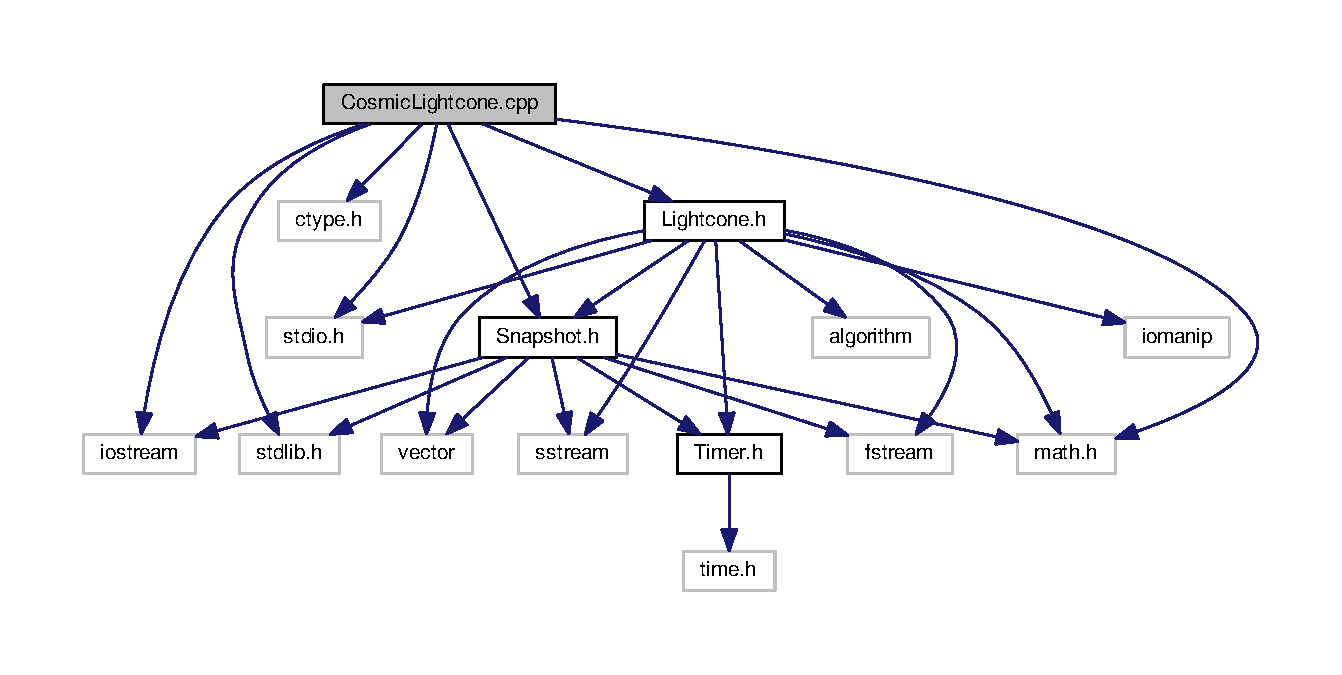
\includegraphics[width=350pt]{CosmicLightcone_8cpp__incl}
\end{center}
\end{figure}
\subsection*{Functions}
\begin{DoxyCompactItemize}
\item 
void \hyperlink{CosmicLightcone_8cpp_afdd7ee29509cd0870f52e020c306fc70}{print\+Spacer} ()
\item 
string \hyperlink{CosmicLightcone_8cpp_ac549e4eaf7118344de33880d88e38543}{get\+String\+From\+User} (string str)
\item 
double \hyperlink{CosmicLightcone_8cpp_a814ce0ea2984e3f9d99029d27b1668e3}{get\+Double\+From\+User} (string str, double max, double min)
\item 
\hyperlink{structLightconeSettings}{Lightcone\+Settings} \hyperlink{CosmicLightcone_8cpp_af81c461b4c952de1a4f9115b17ef7411}{get\+Lightcone\+Settings\+From\+User} ()
\item 
bool \hyperlink{CosmicLightcone_8cpp_aee8048628ff2b5c026c9e15acdcaacb8}{init} ()
\item 
int \hyperlink{CosmicLightcone_8cpp_ae66f6b31b5ad750f1fe042a706a4e3d4}{main} ()
\end{DoxyCompactItemize}


\subsection{Function Documentation}
\hypertarget{CosmicLightcone_8cpp_a814ce0ea2984e3f9d99029d27b1668e3}{}\index{Cosmic\+Lightcone.\+cpp@{Cosmic\+Lightcone.\+cpp}!get\+Double\+From\+User@{get\+Double\+From\+User}}
\index{get\+Double\+From\+User@{get\+Double\+From\+User}!Cosmic\+Lightcone.\+cpp@{Cosmic\+Lightcone.\+cpp}}
\subsubsection[{get\+Double\+From\+User}]{\setlength{\rightskip}{0pt plus 5cm}double get\+Double\+From\+User (
\begin{DoxyParamCaption}
\item[{string}]{str, }
\item[{double}]{max = {\ttfamily 40000}, }
\item[{double}]{min = {\ttfamily 0}}
\end{DoxyParamCaption}
)}\label{CosmicLightcone_8cpp_a814ce0ea2984e3f9d99029d27b1668e3}
\hypertarget{CosmicLightcone_8cpp_af81c461b4c952de1a4f9115b17ef7411}{}\index{Cosmic\+Lightcone.\+cpp@{Cosmic\+Lightcone.\+cpp}!get\+Lightcone\+Settings\+From\+User@{get\+Lightcone\+Settings\+From\+User}}
\index{get\+Lightcone\+Settings\+From\+User@{get\+Lightcone\+Settings\+From\+User}!Cosmic\+Lightcone.\+cpp@{Cosmic\+Lightcone.\+cpp}}
\subsubsection[{get\+Lightcone\+Settings\+From\+User}]{\setlength{\rightskip}{0pt plus 5cm}{\bf Lightcone\+Settings} get\+Lightcone\+Settings\+From\+User (
\begin{DoxyParamCaption}
{}
\end{DoxyParamCaption}
)}\label{CosmicLightcone_8cpp_af81c461b4c952de1a4f9115b17ef7411}
\hypertarget{CosmicLightcone_8cpp_ac549e4eaf7118344de33880d88e38543}{}\index{Cosmic\+Lightcone.\+cpp@{Cosmic\+Lightcone.\+cpp}!get\+String\+From\+User@{get\+String\+From\+User}}
\index{get\+String\+From\+User@{get\+String\+From\+User}!Cosmic\+Lightcone.\+cpp@{Cosmic\+Lightcone.\+cpp}}
\subsubsection[{get\+String\+From\+User}]{\setlength{\rightskip}{0pt plus 5cm}string get\+String\+From\+User (
\begin{DoxyParamCaption}
\item[{string}]{str}
\end{DoxyParamCaption}
)}\label{CosmicLightcone_8cpp_ac549e4eaf7118344de33880d88e38543}
\hypertarget{CosmicLightcone_8cpp_aee8048628ff2b5c026c9e15acdcaacb8}{}\index{Cosmic\+Lightcone.\+cpp@{Cosmic\+Lightcone.\+cpp}!init@{init}}
\index{init@{init}!Cosmic\+Lightcone.\+cpp@{Cosmic\+Lightcone.\+cpp}}
\subsubsection[{init}]{\setlength{\rightskip}{0pt plus 5cm}bool init (
\begin{DoxyParamCaption}
{}
\end{DoxyParamCaption}
)}\label{CosmicLightcone_8cpp_aee8048628ff2b5c026c9e15acdcaacb8}
\hypertarget{CosmicLightcone_8cpp_ae66f6b31b5ad750f1fe042a706a4e3d4}{}\index{Cosmic\+Lightcone.\+cpp@{Cosmic\+Lightcone.\+cpp}!main@{main}}
\index{main@{main}!Cosmic\+Lightcone.\+cpp@{Cosmic\+Lightcone.\+cpp}}
\subsubsection[{main}]{\setlength{\rightskip}{0pt plus 5cm}int main (
\begin{DoxyParamCaption}
{}
\end{DoxyParamCaption}
)}\label{CosmicLightcone_8cpp_ae66f6b31b5ad750f1fe042a706a4e3d4}
\hypertarget{CosmicLightcone_8cpp_afdd7ee29509cd0870f52e020c306fc70}{}\index{Cosmic\+Lightcone.\+cpp@{Cosmic\+Lightcone.\+cpp}!print\+Spacer@{print\+Spacer}}
\index{print\+Spacer@{print\+Spacer}!Cosmic\+Lightcone.\+cpp@{Cosmic\+Lightcone.\+cpp}}
\subsubsection[{print\+Spacer}]{\setlength{\rightskip}{0pt plus 5cm}void print\+Spacer (
\begin{DoxyParamCaption}
{}
\end{DoxyParamCaption}
)}\label{CosmicLightcone_8cpp_afdd7ee29509cd0870f52e020c306fc70}

\hypertarget{Lightcone_8cpp}{}\section{Lightcone.\+cpp File Reference}
\label{Lightcone_8cpp}\index{Lightcone.\+cpp@{Lightcone.\+cpp}}
{\ttfamily \#include \char`\"{}Lightcone.\+h\char`\"{}}\\*
Include dependency graph for Lightcone.\+cpp\+:
\nopagebreak
\begin{figure}[H]
\begin{center}
\leavevmode
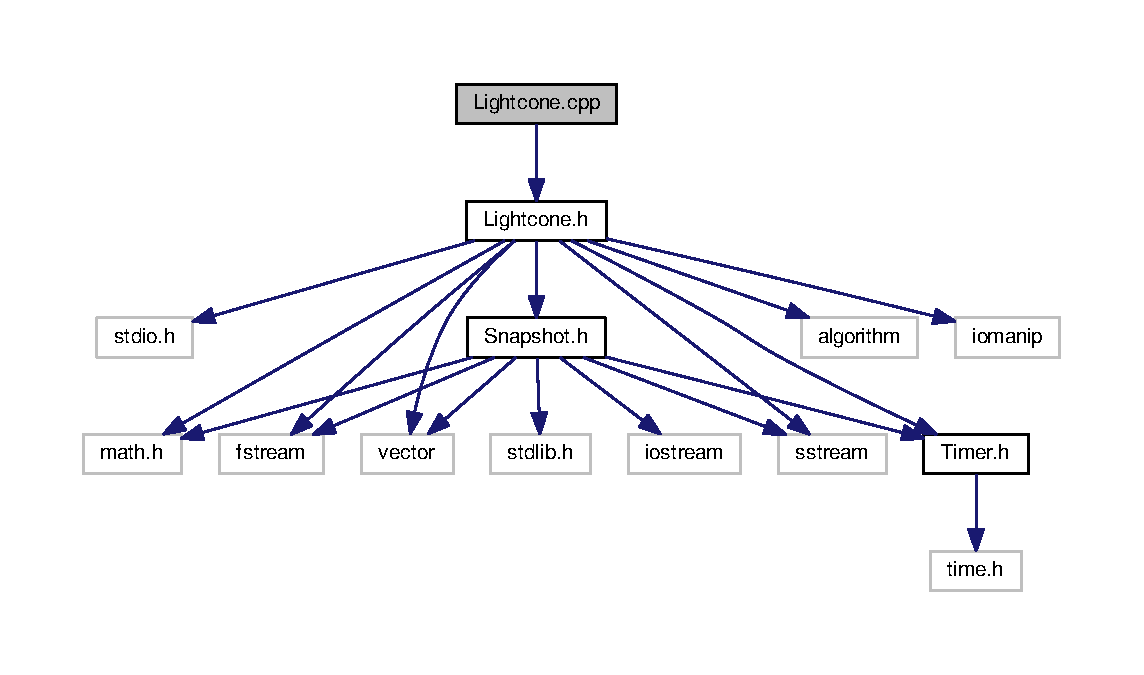
\includegraphics[width=350pt]{Lightcone_8cpp__incl}
\end{center}
\end{figure}

\hypertarget{Lightcone_8h}{}\section{Lightcone.\+h File Reference}
\label{Lightcone_8h}\index{Lightcone.\+h@{Lightcone.\+h}}
{\ttfamily \#include $<$stdio.\+h$>$}\\*
{\ttfamily \#include $<$math.\+h$>$}\\*
{\ttfamily \#include $<$fstream$>$}\\*
{\ttfamily \#include $<$vector$>$}\\*
{\ttfamily \#include $<$algorithm$>$}\\*
{\ttfamily \#include $<$sstream$>$}\\*
{\ttfamily \#include \char`\"{}Snapshot.\+h\char`\"{}}\\*
{\ttfamily \#include \char`\"{}Timer.\+h\char`\"{}}\\*
{\ttfamily \#include $<$iomanip$>$}\\*
Include dependency graph for Lightcone.\+h\+:
\nopagebreak
\begin{figure}[H]
\begin{center}
\leavevmode
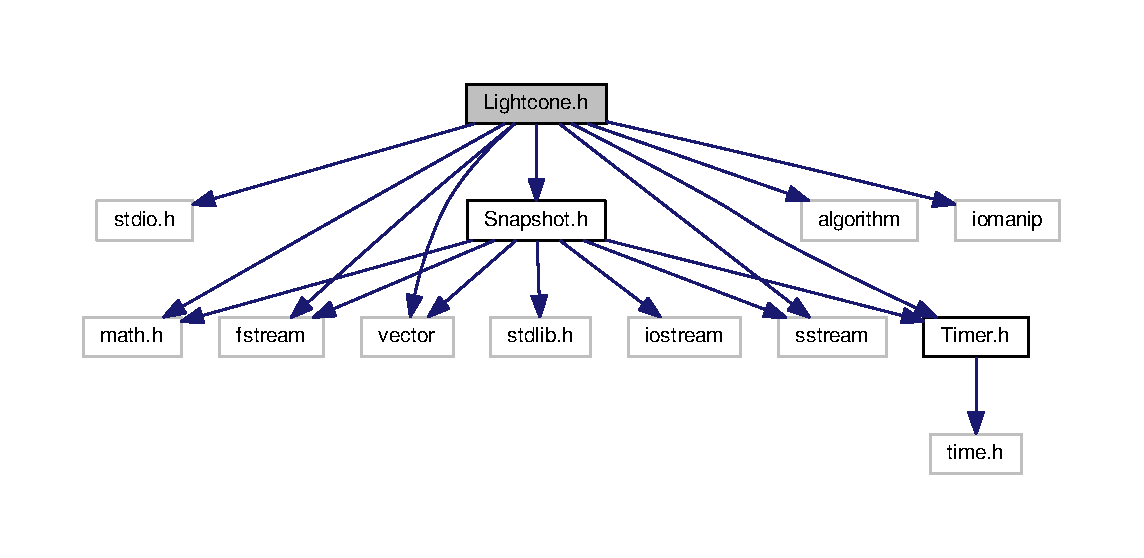
\includegraphics[width=350pt]{Lightcone_8h__incl}
\end{center}
\end{figure}
This graph shows which files directly or indirectly include this file\+:
\nopagebreak
\begin{figure}[H]
\begin{center}
\leavevmode
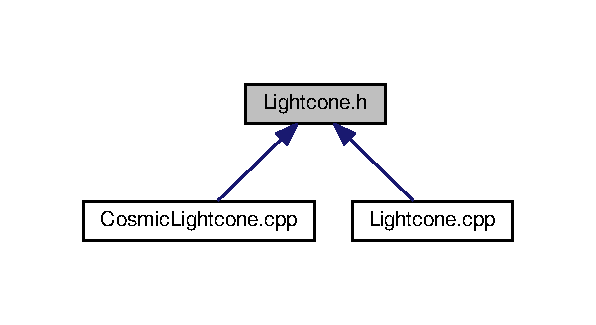
\includegraphics[width=286pt]{Lightcone_8h__dep__incl}
\end{center}
\end{figure}
\subsection*{Classes}
\begin{DoxyCompactItemize}
\item 
struct \hyperlink{structLightconeSettings}{Lightcone\+Settings}
\item 
class \hyperlink{classLightcone}{Lightcone}
\end{DoxyCompactItemize}

\hypertarget{Snapshot_8cpp}{}\section{Snapshot.\+cpp File Reference}
\label{Snapshot_8cpp}\index{Snapshot.\+cpp@{Snapshot.\+cpp}}
{\ttfamily \#include \char`\"{}Snapshot.\+h\char`\"{}}\\*
Include dependency graph for Snapshot.\+cpp\+:
\nopagebreak
\begin{figure}[H]
\begin{center}
\leavevmode
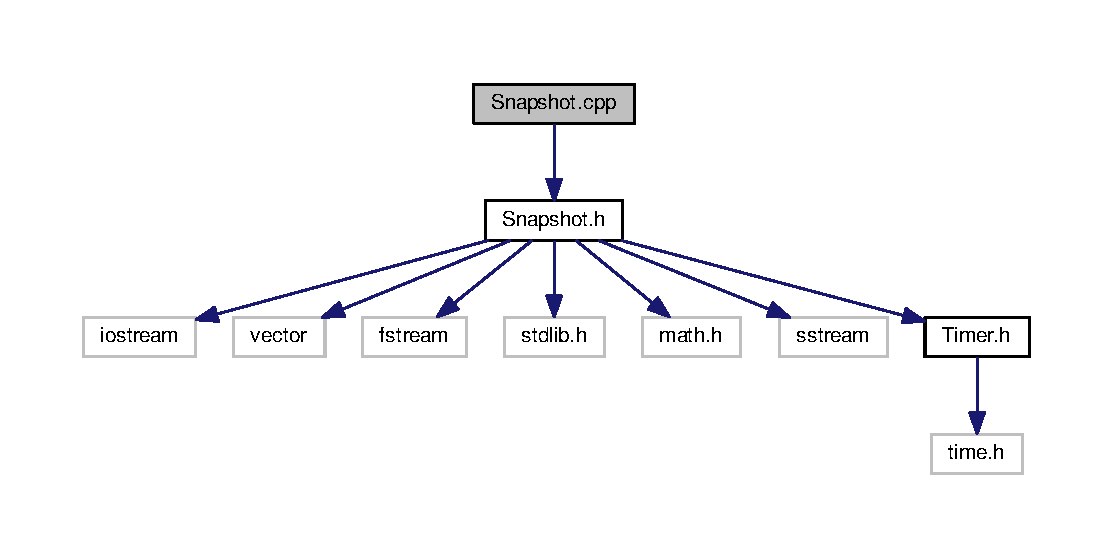
\includegraphics[width=350pt]{Snapshot_8cpp__incl}
\end{center}
\end{figure}

\hypertarget{Snapshot_8h}{}\section{Snapshot.\+h File Reference}
\label{Snapshot_8h}\index{Snapshot.\+h@{Snapshot.\+h}}
{\ttfamily \#include $<$iostream$>$}\\*
{\ttfamily \#include $<$vector$>$}\\*
{\ttfamily \#include $<$fstream$>$}\\*
{\ttfamily \#include $<$stdlib.\+h$>$}\\*
{\ttfamily \#include $<$math.\+h$>$}\\*
{\ttfamily \#include $<$sstream$>$}\\*
{\ttfamily \#include \char`\"{}Timer.\+h\char`\"{}}\\*
Include dependency graph for Snapshot.\+h\+:
\nopagebreak
\begin{figure}[H]
\begin{center}
\leavevmode
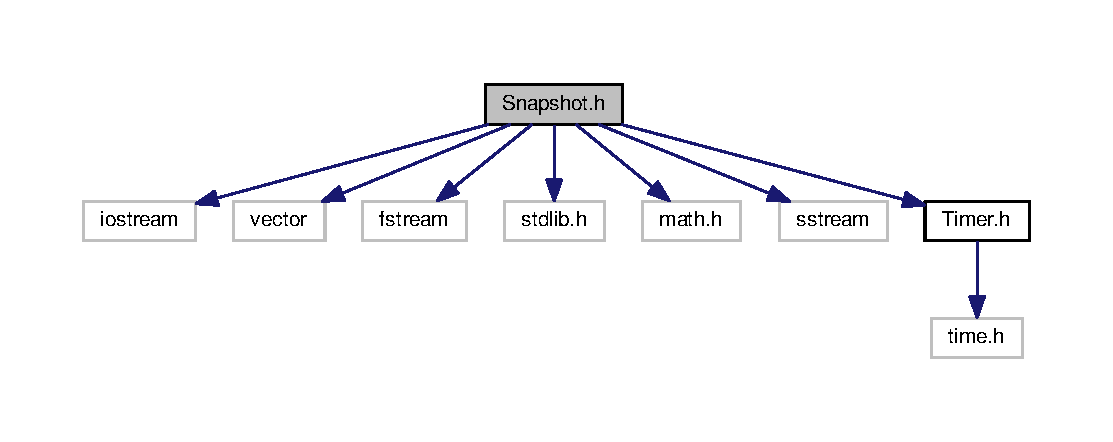
\includegraphics[width=350pt]{Snapshot_8h__incl}
\end{center}
\end{figure}
This graph shows which files directly or indirectly include this file\+:
\nopagebreak
\begin{figure}[H]
\begin{center}
\leavevmode
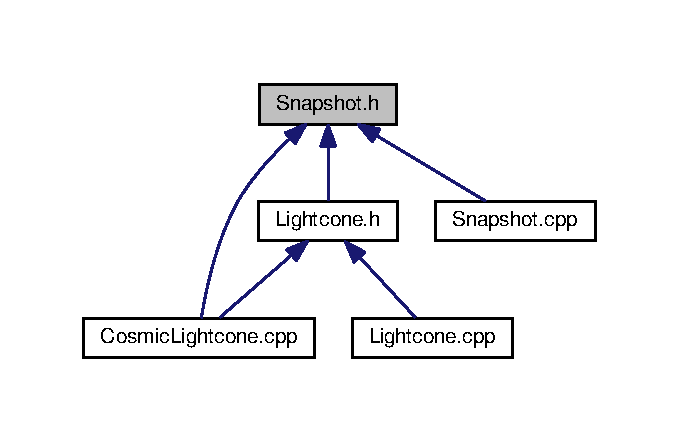
\includegraphics[width=326pt]{Snapshot_8h__dep__incl}
\end{center}
\end{figure}
\subsection*{Classes}
\begin{DoxyCompactItemize}
\item 
struct \hyperlink{structParticle}{Particle}
\item 
struct \hyperlink{structBox}{Box}
\item 
class \hyperlink{classSnapshot}{Snapshot}
\end{DoxyCompactItemize}

\hypertarget{Timer_8cpp}{}\section{Timer.\+cpp File Reference}
\label{Timer_8cpp}\index{Timer.\+cpp@{Timer.\+cpp}}
{\ttfamily \#include \char`\"{}Timer.\+h\char`\"{}}\\*
Include dependency graph for Timer.\+cpp\+:
\nopagebreak
\begin{figure}[H]
\begin{center}
\leavevmode
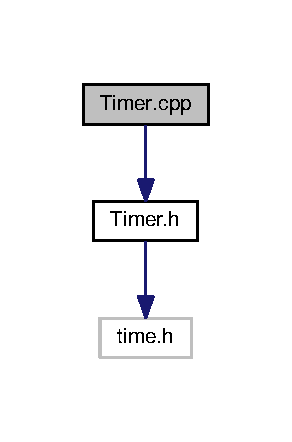
\includegraphics[width=140pt]{Timer_8cpp__incl}
\end{center}
\end{figure}

\hypertarget{Timer_8h}{}\section{Timer.\+h File Reference}
\label{Timer_8h}\index{Timer.\+h@{Timer.\+h}}
{\ttfamily \#include $<$time.\+h$>$}\\*
Include dependency graph for Timer.\+h\+:
\nopagebreak
\begin{figure}[H]
\begin{center}
\leavevmode
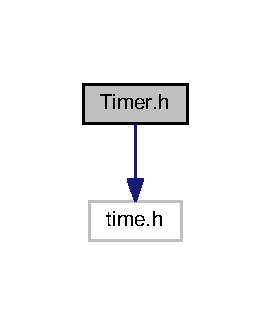
\includegraphics[width=130pt]{Timer_8h__incl}
\end{center}
\end{figure}
This graph shows which files directly or indirectly include this file\+:
\nopagebreak
\begin{figure}[H]
\begin{center}
\leavevmode
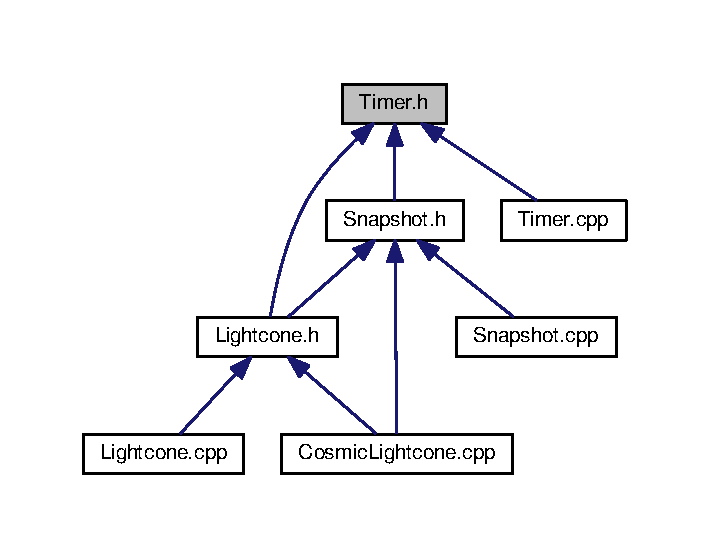
\includegraphics[width=341pt]{Timer_8h__dep__incl}
\end{center}
\end{figure}
\subsection*{Classes}
\begin{DoxyCompactItemize}
\item 
class \hyperlink{classTimer}{Timer}
\end{DoxyCompactItemize}

%--- End generated contents ---

% Index
\backmatter
\newpage
\phantomsection
\clearemptydoublepage
\addcontentsline{toc}{chapter}{Index}
\printindex

\end{document}
